\documentclass[english]{exercise}

\title{Homework 5}
\author{Joshua Feld (406718)}
\professor{Prof. Kowalski}
\course{Partial Differential Equations}

\begin{document}
    \maketitle


    \section{}

    \begin{quote}
        Consider the following one-dimensional boundary value problem
        \begin{align*}
            -u''\parentheses*{x} + u\parentheses*{x} &= f\parentheses*{x}, \quad \text{in }\parentheses*{0, 1} \subset \R,\\
            u\parentheses*{0} &= 0 \quad \text{(Dirichlet)},\\
            \alpha u\parentheses*{1} + u'\parentheses*{1} &= a, \quad \alpha \ge 0, a \in \R \quad \text{(Robin)}.
        \end{align*}
        \begin{enumerate}
            \item Derive the weak formulation of the above problem.
            \item Find the discrete solution using the finite element method.
            Choose the continuous piecewise linear functions
            \[
                \psi_i\parentheses*{x} := \begin{cases}
                    \frac{x - x_{i - 1}}{h_i}, & \text{if }x \in I_i = \parentheses*{x_{i - 1}, x_i},\\
                    \frac{x_{i + 1} - x}{h_{i + 1}}, & \text{if }x \in I_{i + 1} = \parentheses*{x_i, x_{i + 1}},\\
                    0, & \text{otherwise}
                \end{cases}
            \]
            as basis functions on a uniform grid, \(0 = x_0 < \cdots < x_N = 1\) with \(h = x_i - x_{i - 1}\).
        \end{enumerate}
    \end{quote}
    
    \begin{enumerate}
        \item Consider the test function \(v \in V_0\),where the space \(V_0\) is defined by
        \[
            V_0 = \braces*{u \in H\parentheses*{0, 1} : u\parentheses*{0} = 0}.
        \]
        Multiplying the given differential equation by \(v \in V_0\) and integrating over the domain \(\parentheses*{0, 1}\), we get
        \begin{align*}
            -\int_0^1 u''v\d x + \int_0^1 uv\d x &= \int_0^1 fv\d x\\
            \iff \int_0^1 u'v'\d x - u'\parentheses*{1}v\parentheses*{1} + \int_0^1 uv\d x &= \int_0^1 fv\d x\\
            \iff \int_0^1 u'v'\d x - \parentheses*{a - \alpha u\parentheses*{1}}v\parentheses*{1} + \int_0^1 uv\d x &= \int_0^1 fv\d x\\
            \iff \int_0^1 u'v'\d x + \int_0^1 uv\d x + \alpha u\parentheses*{1}v\parentheses*{1} &= \int_0^1 fv\d x + av\parentheses*{1}.
        \end{align*}
        The weak formulation is given by:
        \begin{quote}
            ``Find \(u \in V_0\) such that
            \[
                a\parentheses*{u, v} = \ell\parentheses*{v} \quad \forall v \in V_0\parentheses*{0, 1}
            \]
            where
            \begin{align*}
                a\parentheses*{u, v} &= \int_0^1 u'v'\d x + \int_0^1 uv\d x + \alpha u\parentheses*{1}v\parentheses*{1},\\
                \ell\parentheses*{v} &= \int_0^1 fv\d x + av\parentheses*{1}.\text{''}
            \end{align*}
        \end{quote}
        \item Let \(u_h \in V_h \subset V_0\parentheses*{0, 1}\) be an approximate solution of the given boundary value problem.
        Here, \(V_h\) is the space of continuous, piecewise linear functions, defined by
        \[
            V_h = \braces*{u \in C^0\parentheses*{\brackets*{0, 1}} : \left.u\right|_{I_i} \in P_1, i = 1, \ldots, N, u\parentheses*{0} = 0}.
        \]
        A basis of \(V_h\) is given by the basis functions \(\psi_i\parentheses*{x_j} = \delta_{ij}\),
        \[
            \psi_i\parentheses*{x} = \begin{cases}
                \frac{x - x_{i - 1}}{h_i}, & \text{if }x \in I_i = \parentheses*{x_{i - 1}, x_i},\\
                \frac{x_{i + 1} - x}{h_{i + 1}}, & \text{if }x \in I_{i + 1} = \parentheses*{x_i, x_{i + 1}},\\
                0, & \text{otherwise}.
            \end{cases}
        \]
        The discrete solution is given by
        \[
            u_h\parentheses*{x} = \sum_{i = 1}^N c_i \psi_i.
        \]
        The discrete weak formulation is given by
        \begin{align*}
            \sum_{i = 1}^N a\parentheses*{\psi_i, \psi_j}c_i &= b_j \quad \forall j = 1, \ldots, N,\\
            Ac &= b
        \end{align*}
        where
        \begin{align*}
            A_{i, j} &= a\parentheses*{\psi_i, \psi_j} = \int_0^1 \psi_i'\psi_j'\d x + \int_0^1 \psi_i \psi_j \d x + \alpha\psi_i\parentheses*{1}\psi_j\parentheses*{1},\\
            b_j &= \int_0^1f\psi_j \d x + a\psi_j\parentheses*{1}.
        \end{align*}
        The values of \(\int_0^1 \psi_i'\psi_j'\d x\) and \(\int_0^1 \psi_i \psi_j \d x\) are given by
        \[
            \int_0^1 \psi_i'\psi_j'\d x = \begin{cases}
                \frac{2}{h}, & \text{if }i = j,\\
                -\frac{1}{h}, & \text{if }j = i \pm 1,\\
                0, & \text{otherwise},
            \end{cases} \quad \int_0^1 \psi_i \psi_j \d x = \begin{cases}
                \frac{2h}{3}, & \text{if }i = j,\\
                \frac{h}{6}, & \text{if }j = i \pm 1,\\
                0, & \text{otherwise}.
            \end{cases}
        \]
        The values of \(a\parentheses*{\psi_i, \psi_j}\) for \(i, j = 1, \ldots, N - 1\) are given by
        \[
            a\parentheses*{\psi_i, \psi_j} = \begin{cases}
                \frac{2}{h} + \frac{2h}{3}, & \text{if }i = j,\\
                -\frac{1}{h} + \frac{h}{6}, & \text{if }j = i \pm 1,\\
                0, & \text{otherwise}
            \end{cases}
        \]
        while \(a\parentheses*{\psi_{N - 1}, \psi_N}\), \(a\parentheses*{\psi_N, \psi_{N - 1}}\) and \(a\parentheses*{\psi_N, \psi_N}\) are given by
        \[
            a\parentheses*{\psi_{N - 1}, \psi_N} = a\parentheses*{\psi_N, \psi_{N - 1}} = -\frac{1}{h} + \frac{h}{6}, \quad a\parentheses*{\psi_N, \psi_N} = \frac{1}{h} + \frac{h}{3} + \alpha.
        \]
        From this it is clear that the stiffness matrix \(A\) is tridiagonal.
        The values of \(b_j\) are given by
        \[
            b_j = \begin{cases}
                \int_{x_j - 1}^{x_j + 1}f\psi_j\d x, & \text{if }j = 1, \ldots, N - 1,\\
                \int_{x_j - 1}^{x_j}f\psi_j\d x + a, & \text{if }j = N.
            \end{cases}
        \]
        The discrete solution is obtained by solving the linear system of equations
        \[
            \sum_{i = 1}^N a\parentheses*{\psi_i, \psi_j}c_i = b_j \quad \forall j = 1, \ldots, N.
        \]
    \end{enumerate}
    
    
    \section{}
    
    \begin{quote}
        We again consider the one-dimensional Poisson problem
        \begin{align*}
            -u''\parentheses*{x} &= f\parentheses*{x}, \quad \text{in }\parentheses*{0, 1},\\
            u\parentheses*{0} = u\parentheses*{1} &= 0.
        \end{align*}
        The domain \(\Omega := \parentheses*{0, 1}\) is equipped with the grid \(0 = x_0 < \cdots < x_N = 1\).
        In contrast to the previous task, we now consider the approximation space \(V_h\) of continuous, piecewise quadratic functions, i.e.,
        \[
            V_h = \braces*{u \in C^0\parentheses*{\brackets*{0, 1}} : u_{\brackets*{x_{k - 1}, x_k}} = a_k + b_k x + c_k x^2, k = 1, \ldots, N, u\parentheses*{0} = u\parentheses*{1} = 0}.
        \]
        We equip this space with basis functions of the form displayed in Figure \ref{fig:2-1}.
        \begin{figure}[ht]
            \centering
            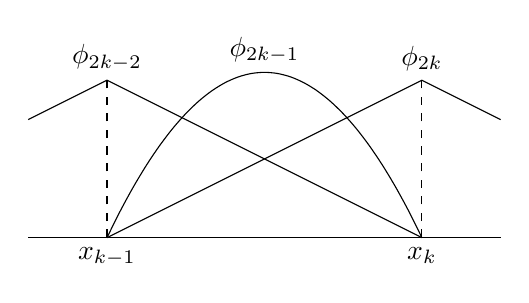
\begin{tikzpicture}
                \draw (0,0) -- (6,0);
                \node[anchor=north] at (1,0) {\(x_{k - 1}\)};
                \node[anchor=north] at (5,0) {\(x_k\)};
                \draw[dashed] (1,0) -- (1,2);
                \draw[dashed] (5,0) -- (5,2);
                \draw (0,1.5) -- (1,2) -- (5,0);
                \draw (1,0) -- (5,2) -- (6,1.5);
                \draw[domain=1:5, smooth, variable=\x] plot ({\x}, {-21/40*\x*\x + 63/20*\x - 21/8});
                \node[anchor=south] at (1,2) {\(\phi_{2k - 2}\)};
                \node[anchor=south] at (3,2.1) {\(\phi_{2k - 1}\)};
                \node[anchor=south] at (5,2) {\(\phi_{2k}\)};
            \end{tikzpicture}
            \caption{Piecewise quadratic basis functions}
            \label{fig:2-1}
        \end{figure}
        To be precise the basis consists of the usual \(N - 1\) hat functions \(\braces*{\phi_{2k}}_{k = 1}^{N - 1}\) together with an additional \(N\) functions \(\braces*{\phi_{2k - 1}}_{k = 1}^N\) defined as
        \[
            \phi_{2k - 1}\parentheses*{x} = \begin{cases}
                a + bx + cx^2, & \text{if }x \in \parentheses*{x_{k - 1}, x_k}\text{ with }\phi_{2k - 1}\parentheses*{\frac{x_{k - 1} + x_k}{2}} = 1,\\
                0, & \text{otherwise}.
            \end{cases}
        \]
        Write down the Galerkin discretization of this problem for the approximation space \(V_h\).
        Compute the stiffness matrix \(A\) using the definition of the basis \(\braces*{\phi_i}_{i = 1}^{2N - 1}\) of hat functions.
        Show your computations.
    \end{quote}

    Galerkin discretization:
    Find \(u_h \in V_h\) such that for all test functions \(v_h \in V_h\) it holds that
    \[
        a\parentheses*{u_h, v_h} := \int_0^1 u_h'\parentheses*{x}v_h'\parentheses*{x}\d x = \int_0^1 f\parentheses*{x}v_h\parentheses*{x}\d x =: \ell\parentheses*{v_h}.
    \]
    We denote the basis functions on this space by \(\braces*{\phi_i}_{i = 1}^{2N - 1}\).
    The Galerkin discretization then results in a stiffness matrix \(A\) with entries of the form \(A_{i, j} = \sum_{k = 1}^N A_{i, j}^{\parentheses*{k}}\), where the element matrices \(A_{i,j}^{\parentheses*{k}}\) are given by
    \[
        A_{i, j}^{\parentheses*{k}} = \int_{I_k} \phi_i'\phi_j'\d x.
    \]
    Here, \(I_k\) denotes the interval \(\parentheses*{x_{k - 1}, x_k}\).
    
    In order to evaluate these integrals, we will map the sub-interval \(I_k\) to the reference interval \(\parentheses*{0, 1}\).
    To this end, we define \(a := x_{k - 1}, b:= x_k, h_k := b - a\).
    Furthermore, we introduce the substitution \(x = a + h_k y, \d x = h_k \d y\), and we define the functions
    \[
        \hat{\phi}_1\parentheses*{y} := 1 - y, \quad \hat{\phi}_2\parentheses*{y} := 4\parentheses*{1 - y}y, \quad \hat{\phi}_3\parentheses*{y} := y
    \]
    for all \(y \in \parentheses*{0, 1}\).
    It can now be seen that
    \begin{align*}
        \int_{I_k}\phi_{2k - 2}'\phi_{2k - 2}'\d x &= \frac{1}{h_k}\int_0^1 \hat{\phi}_1'\parentheses*{y}\hat{\phi}_1'\parentheses*{y}\d y = \frac{1}{h_k},\\
        \int_{I_k}\phi_{2k}'\phi_{2k}'\d x &= \frac{1}{h_k}\int_0^1 \hat{\phi}_3'\parentheses*{y}\hat{\phi}_3'\parentheses*{y}\d y = \frac{1}{h_k},\\
        \int_{I_k}\phi_{2k - 1}'\phi_{2k - 1}'\d x &= \frac{1}{h_k}\int_0^1 \hat{\phi}_2'\parentheses*{y}\hat{\phi}_2'\parentheses*{y}\d y = \frac{1}{h_k}\int_0^1 \parentheses*{4 - 8y}^2\d y = \frac{1}{h_k}\frac{16}{3},\\
        \int_{I_k}\phi_{2k - 2}'\phi_{2k}'\d x &= \frac{1}{h_k}\int_0^1 \hat{\phi}_1'\parentheses*{y}\hat{\phi}_3'\parentheses*{y}\d y = -\frac{1}{h_k},\\
        \int_{I_k}\phi_{2k - 2}'\phi_{2k - 1}'\d x &= \frac{1}{h_k}\int_0^1 \hat{\phi}_1'\parentheses*{y}\hat{\phi}_2'\parentheses*{y}\d y = -\frac{1}{h_k}\int_0^1 \parentheses*{4 - 8y}\d y = 0,\\
        \int_{I_k}\phi_{2k}'\phi_{2k - 1}'\d x &= \frac{1}{h_k}\int_0^1 \hat{\phi}_3'\parentheses*{y}\hat{\phi}_2'\parentheses*{y}\d y = \frac{1}{h_k}\int_0^1 \parentheses*{4 - 8y}\d y = 0.
    \end{align*}
    Using these computations, we obtain the following stiffness matrix
    \[
        A = \begin{pmatrix}
            \frac{1}{h_1}\frac{16}{3} & 0 & 0 & 0 & \cdots & \cdots & 0\\
            0 & \frac{1}{h_1} + \frac{1}{h_2} & 0 & -\frac{1}{h_2} & \ddots & & \vdots\\
            0 & 0 & \frac{1}{h_2}\frac{16}{3} & \ddots & \ddots & \ddots & \vdots\\
            0 & -\frac{1}{h_2} & \ddots & \ddots & \ddots & -\frac{1}{h_{N - 1}} & 0\\
            \vdots & \ddots & \ddots & \ddots & \frac{1}{h_{N - 1}}\frac{16}{3} & 0 & 0\\
            \vdots & & \ddots & -\frac{1}{h_{N - 1}} & 0 & \frac{1}{h_{N - 1}} + \frac{1}{h_N} & 0\\
            0 & \cdots & \cdots & 0 & 0 & 0 & \frac{1}{h_N}\frac{16}{3}
        \end{pmatrix}.
    \]
    If we further assume that \(h = h_k\), then we obtain that
    \[
        A = \frac{1}{h}\begin{pmatrix}
            \frac{16}{3} & 0 & 0 & 0 & \cdots & \cdots & 0\\
            0 & 2 & 0 & -1 & \ddots & & \vdots\\
            0 & 0 & \frac{16}{3} & \ddots & \ddots & \ddots & \vdots\\
            0 & -1 & \ddots & \ddots & \ddots & -1 & 0\\
            \vdots & \ddots & \ddots & \ddots & \frac{16}{3} & 0 & 0\\
            \vdots & & \ddots & -1 & 0 & 2 & 0\\
            0 & \cdots & \cdots & 0 & 0 & 0 & \frac{16}{3}
        \end{pmatrix}.
    \]
\end{document}
